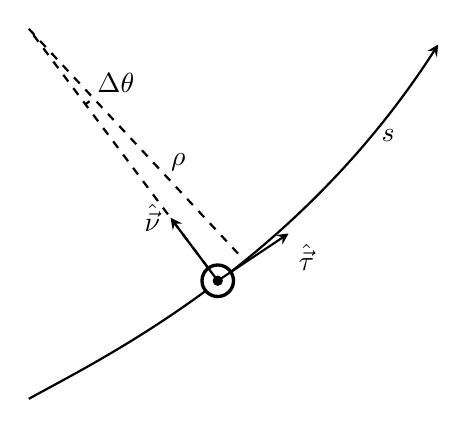
\begin{tikzpicture}[>=stealth, scale=1.0]

    % % Background ruled lines
    % \foreach \y in {-2,-1,0,1,2,3} {
    %     \draw[gray!30, very thin] (-4,\y) -- (4,\y);
    % }

    % Path S
    \draw[thick, ->] (-2.4,-1.5) .. controls (-1.5,-1.0) and (1.0,0.2) .. (2.8, 3.0) node[pos=0.85, right] {\(s\)};

    % Dashed lines
    % Extension of velocity vector
    \draw[dashed, thick] (0,0) -- (-2.4, 3.2); 
    % Line towards center of curvature P
    \draw[dashed, thick] (-2.4, 3.2) -- (0.3,0.3) ; 

    % Angle Delta Theta
    % Angle of v extension: atan2(3.2, -2.4) = 126.87 degrees
    % Angle of P line: atan2(2.7, 1.6) = 59.35 degrees
    \draw[thick] (-2.4,3.2) ++(126.87:-1.2) arc (126.87:130:-1.2) node[pos=0.4, above right] {\(\Delta \theta\)};

    % Particle (circle with inner dot)
    \draw[very thick, fill=white] (0,0) circle (0.2);
    \filldraw[thick] (0,0) circle (0.05); 

    % Velocity vector v
    \draw[->, thick] (0,0) -- (-0.6, 0.8) node[left] {\(\hat{\vec{\nu}}\)};

    % Change in velocity vector Delta v
    \draw[->, thick] (0,0) -- (0.9, 0.6) node[below right] {\(\hat{\vec{\tau}}\)};

    % % Angle beta
    % % Tangent backward angle: atan2(-1.6, 1.2) = -53.13 degrees
    % \draw[thick] (0,0) ++(0:0.6) arc (0:-53.13:0.6);
    \node at (-0.5,1.5) {\(\rho\)};

\end{tikzpicture}